\section{Additional material on Section~\ref{sec:trending}}\label{sec:appendix-trending}

\subsection{Data generation for Section~\ref{sec:trending}}\label{subsec:app-trending-data-generation}

The first dataset is generated by sequentially generating $\diffx$ and $\diffy$.
First, the $\diffxt$ are sampled as a sum of a standard normal random number and a uniform random number on $(-10, 10)$:
\begin{equation*}
    \diffxt \sim N(0, 1) + U(-10, 10) \quad t = 1, \dots, T.
\end{equation*}
Subsequently, the $\diffy$ are simulated for a constant trending ratio $k$ by
\begin{equation*}
    \diffyt = \diffxt \cdot n_t \cdot b_t,
\end{equation*}
where $n_t$ is a truncated normal distribution with mean one and standard deviation 0.5, truncated at 0, and $b_t$ is a symmetric Bernoulli random variable with parameter $k$.
For a time-varying trending ratio, the parameter $k$ is modified to have a wave-shape over time, that is,
\begin{equation*}
    k_t = 0.75 + \sin(t / 365.25 \cdot 2 \pi) / 4.
\end{equation*}
For the asymmetric trending ratio, $k$ is a function of $\diffxt$,
\begin{equation*}
    k(x) = 0.5 + \min \left\{ \max \left\{ \frac{x + 5}{10}, 0  \right\} , 1 \right\} / 2.
\end{equation*}

In the second approach, $\diffyt$ and $\diffxt$ are modeled to be multivariate normal with mean 0 and covariance matrix
\begin{equation*}
    \Sigma = \begin{pmatrix} 4 & 3 \\ 3 & 4 \end{pmatrix}.
\end{equation*}
Thus, the conditional probability of trending can be calculated by a conditional normal distribution to
\begin{equation*}
    P(\diffyrv \diffxrv > 0 | \diffxrv = x) = \Phi \left( \frac{3}{2 \sqrt{7}} x \right),
\end{equation*}
where $\Phi$ is a standard normal \ac{cdf}.

The four-quadrant plots for the sample realizations of the data generation schemes are shown in Figure~\ref{fig:appendix_dgps}.

\begin{figure}
    \centering
    \begin{subfigure}{0.24\textwidth}
        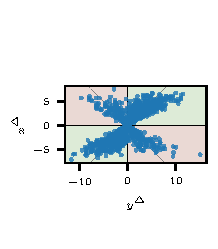
\includegraphics{plots/illustrative_examples/appendix_4q_dgp1}
        \caption{Constant trending ratio.}
    \end{subfigure}\hspace{0.01\textwidth}
    \begin{subfigure}{0.24\textwidth}
        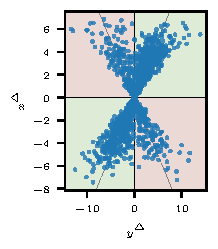
\includegraphics{plots/illustrative_examples/appendix_4q_dgp1_time}
        \caption{Time-varying trending ratio}
    \end{subfigure}\hspace{0.01\textwidth}
    \begin{subfigure}{0.24\textwidth}
        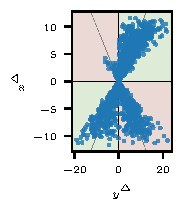
\includegraphics{plots/illustrative_examples/appendix_4q_dgp1_asym}
        \caption{Asymmetric trending ratio}
    \end{subfigure}\hspace{0.01\textwidth}
    \begin{subfigure}{0.24\textwidth}
        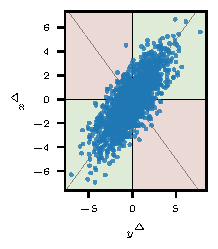
\includegraphics{plots/illustrative_examples/appendix_4q_dgp2}
        \caption{Second approach}
    \end{subfigure}
    \caption{Four-quadrant plots for sample realizations of the data generation schemes of Section~\ref{subsec:app-trending-data-generation}. Although the first and second plots differ over time, their difference is not discernible in the plots. The third data set's asymmetry is visible in the plot, but the decrease in the trending ability near 0 is not visible. }
    \label{fig:appendix_dgps}
\end{figure}

\subsection{Simulation study on bootstrapping confidence intervals}\label{subsec:appendix-trending-bootstrap}


We examine three methods for bootstrapping: the intuitive percentile and the more sophisticated basic and \ac{bca} method.
In the \textit{percentile} approach, the confidence interval for the level $\alpha$ is built directly from the empirical distribution of the bootstrap estimators.
The \textit{basic} approach computes the confidence interval based on the non-bootstrap estimate using the bootstrapped quantile deviations~\citep{Davison1997}.
The \ac{bca} method modifies the quantiles of the empirical bootstrap distribution by a bias and an acceleration parameter~\citep{Efron1987}.
Typically, the percentile approach needs larger datasets and provides an easy and fast estimate, while the \ac{bca} is computationally expensive but requires smaller datasets for reasonable confidence intervals.
The basic approach balances these two objectives.
We compare the approaches in a small synthetic data study on their small-dataset behavior and computation time.

We vary the number of available time steps $T$ to be a typical time-series value, such as 30 for daily data in a month, 52 for weekly data, 168, 365, 720, and 1024.
The considered datasets are the first dataset with asymmetric dependence and the second dataset outlined in Appendix~\ref{subsec:app-trending-data-generation}.
In the calculations, the \verb|scipy| package's implementation of bootstrap confidence intervals is used~\citep{Virtanen2020}.
The prescribed confidence level is 90 \%, and the number of bootstrap samples is $10,000$.
The share of confidence intervals covering the true values per method and $T$ are shown in Table~\ref{tab:trending_bootstrap}.
The true values of the accuracy are computed based on a dataset of size $10^8$, yielding 0.7501 and 0.7700 for the two datasets.
The computation times per method and dataset are shown in Figure~\ref{fig:trending_bootstrap_time}.
For the small sample sizes up to $T = 168$, only the \ac{bca} method keeps the confidence interval size and yields slightly wider confidence intervals.
The method's results do not differ for the larger sample sizes.
The computation time for the \ac{bca} method is slightly larger than for the other methods, but all methods have a moderate computation time.
\Ac{bca} is the only method that maintains the confidence level for small datasets while increasing the computation time only moderately for larger datasets.
Therefore, we use the \ac{bca} method for confidence intervals in the applications in Section~\ref{sec:application}.


\begin{table}
    \centering
    \begin{subtable}{.48\textwidth}
        \begin{tabular}{llll}
\toprule
 & percentile & basic & bca \\
\midrule
30 & 0.84 (0.249) & 0.86 (0.250) & 0.91 (nan) \\
52 & 0.89 (0.194) & 0.89 (0.193) & 0.89 (0.198) \\
168 & 0.91 (0.109) & 0.90 (0.109) & 0.90 (0.110) \\
365 & 0.90 (0.074) & 0.90 (0.074) & 0.90 (0.074) \\
720 & 0.90 (0.053) & 0.90 (0.053) & 0.90 (0.053) \\
1024 & 0.90 (0.044) & 0.90 (0.044) & 0.89 (0.044) \\
\bottomrule
\end{tabular}

        \caption{First dataset}
    \end{subtable}\hspace{0.02\textwidth}
    \begin{subtable}{.48\textwidth}
        \begin{tabular}{llll}
\toprule
 & percentile & basic & BCa \\
\midrule
30 & 0.87 (0.243) & 0.88 (0.242) & 0.92 (0.249) \\
52 & 0.87 (0.188) & 0.89 (0.188) & 0.90 (0.192) \\
168 & 0.89 (0.106) & 0.90 (0.106) & 0.90 (0.107) \\
365 & 0.90 (0.072) & 0.90 (0.072) & 0.90 (0.072) \\
720 & 0.90 (0.052) & 0.90 (0.052) & 0.90 (0.052) \\
1024 & 0.89 (0.043) & 0.90 (0.043) & 0.90 (0.043) \\
\bottomrule
\end{tabular}

        \caption{Second dataset}
    \end{subtable}
    \caption{Proportion of bootstrapping confidence intervals covering the true value of trending ratio per method and sample size $T$. The average width of the confidence interval is listed in brackets.}
    \label{tab:trending_bootstrap}
\end{table}

\begin{figure}
    \centering
    \begin{subfigure}{0.48\textwidth}
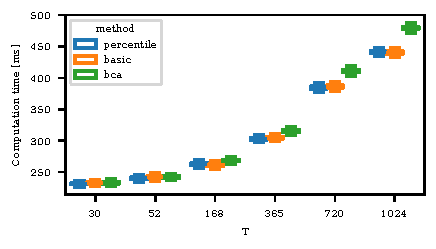
\includegraphics{plots/illustrative_examples/boxplot_comp_time_butterfly}
        \caption{First dataset}
    \end{subfigure}
    \begin{subfigure}{0.48\textwidth}
    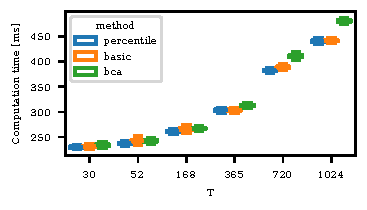
\includegraphics{plots/illustrative_examples/boxplot_comp_time_normal}
        \caption{Second dataset}
    \end{subfigure}
    \caption{Boxplot of the computation time of the different bootstrapping method and data set sizes $T$. The computation time refers to bootstrapping one confidence interval based upon $10,000$ values. Each boxplot reflects $10,000$ samples. The \ac{bca} method takes slightly longer than the other two, but the difference is negligible.}
    \label{fig:trending_bootstrap_time}
\end{figure}


\subsection{Visualization of different bandwidth selectors in multivariate \ac{kde}}\label{subsec:appendix-kde}

We examine the resulting conditional trending plots for the three well-known selectors, rule-of-thumb, cross-validation maximum likelihood, and cross-validation least squares using the \verb|statsmodels| Python package~\citep{Seabold2010} in Figure~\ref{fig:trending-cond-prob-bw}.
While the rule-of-thumb is based only on the covariance matrix, the other two numerically optimize the bandwidth with a hold-one-out least squares or likelihood objective function.
The dashed line shows the theoretical $P(\diffyrv \diffxrv > 0 | \diffxrv = x)$.
The second method, cross-validation least squares, requires long computation times while yielding small or no bandwidth results, even for two relatively small datasets.
The rule-of-thumb and cross-validation maximum likelihood methods yield reasonable results at moderate computation times. 
Further examples, including comparisons between methods regarding their trending ability, are available in Section~\ref{sec:application}.

\begin{figure}
    \centering
    \begin{subfigure}{.48\textwidth}
        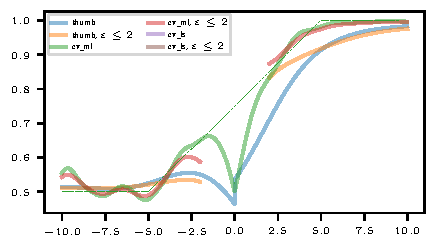
\includegraphics{plots/illustrative_examples/cond_prob_plot_bw_asym_butterfly}
        \caption{First dataset with asymmetric dependence.}
    \end{subfigure}
    \begin{subfigure}{.48\textwidth}
        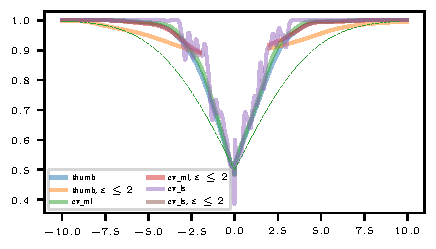
\includegraphics{plots/illustrative_examples/cond_prob_plot_bw_normal}
        \caption{Second dataset. }
    \end{subfigure}
    \caption{Resulting conditional trending plot for different bandwidth selection processes. Cross-validation least squares takes a considerably larger computation time. It does not converge for the first data set and yields a bandwidth too small for the second data set. The rule of thumb is the fastest method but tends to oversmooth. The cross-validation maximum likelihood method yields a more reasonable bandwidth with moderate computation time. $\varepsilon$ specifies an exclusion area $E = \{(x, y) \in \R^2: (-\varepsilon \leq x \leq \varepsilon)\}$ in $\diffx$-direction.}\label{fig:trending-cond-prob-bw}
\end{figure}




\subsection{Probabilistic trending evaluation}

If forecasts or nowcasts are given as quantiles, $p_t$ can be determined by interpolations among the quantiles.
Let $q_p$ denote the quantiles for forecast time $t+l$ for even-spaced probabilities $p \in \{1/\pmax, \dots, (p-1) / \pmax\}$ ($\pmax \in \N \setminus \{1, 2\}$) and $y_t$ the true value at time $t$.
The quantiles $q_p$ generally differ for each time step, but we omit an index here for ease of notation.
The probability $\pc_t$ of a \textit{negative} change is between $p^{\star}$ and $p^{\star} + 1/\pmax$ for
\begin{equation*}
    p^{\star} = \max \{p \in \{1/\pmax, \dots, (\pmax-1) / \pmax\}: q_p \leq y_t\} , \quad \text{if}\ q_{1/\pmax} \leq y_t \leq q_{1 - 1/\pmax}.
\end{equation*}
Quantiles do not determine the location within the interval $[p^{\star}, p^{\star} + 1/\pmax]$.
Under the assumption of a uniform distribution within the quantile interval, the probability of a negative change is
\begin{equation*}
    \pc_t = \frac{y_t - q_{p^\star}}{\pmax (q_{p^{\star} + 1} - q_{p^{\star}})} + p^{\star}.
\end{equation*}
The approach does not assign probabilities for $y_t$ smaller than the smallest quantile $q_{1/p}$ or larger than the largest quantile.
As a simple extension, we assume that the probability mass is uniformly distributed on an interval of the same length as the nearest interval specified by the quantiles.
This yields
\begin{equation*}
\pc_t = \begin{cases}
    \max \{\frac{1}{\pmax} - \frac{q_{p^\star} - y_t}{\pmax (q_{p2/\pmax} - q_{1/\pmax})}, 0\} &, \text{if } y_t < q_{1/p}, \\
    \min \{\frac{1}{\pmax} - \frac{y_t - q_{(\pmax-1)/\pmax}}{\pmax (q_{(\pmax-1)/\pmax} - q_{(\pmax-2)/\pmax})}, 1\} &, \text{if } y_t > q_{1 - 1/p}, \\
    \frac{y_t - q_{p^\star}}{\pmax (q_{p^{\star} + 1} - q_{p^{\star}})} + p^{\star} &, \text{otherwise.}
\end{cases}
\end{equation*}
The probability of positive change is $p_t = 1 - \pc_t$.

If the true value is given as a distribution because it is still unknown, the probabilities $p_t$ can be computed by integration.
Let for two nowcasts the distributions be given by \acp{pdf} $f_{t+l|t+l}$ and $f_{t|t+l}$ with \acp{cdf}  $F_{t+l|t+l}$ and $F_{t|t+l}$.
Then, the probability of a negative change can be computed by
\begin{align}
    \pc_t
        &= \int_{\begin{subarray}{l}x_1, x_2 \in \R: \\ x_2 < x_1\end{subarray}} f_{t|t+l} (x_1) f_{t+l|t+l} (x_2)  \ \textrm{d} \: (x_1, x_2) \nonumber\\
        &= \int_{x_1 \in \R} \int_{-\infty}^{x_1} f_{t|t+l} (x_1) f_{t+l|t+l} (x_2)  \ \textrm{d} \: x_2 \ \textrm{d} \: x_1 \nonumber\\
        &= \int_{x_1 \in \R} f_{t|t+l} (x_1) F_{t+l|t+l} (x_1)  \ \textrm{d} \: x_2 \ \textrm{d} \: x_1 \label{eq:trending-probabilistic-pdf}.
\end{align}
Thereby, the distributions are assumed to be independent.
If the nowcasts have the form of a multivariate distribution, including the dependence of the two \acp{pdf}, $f_{t+l|t+l} (x_2)$ has to be replaced by the \ac{pdf} conditional on $x_1$.
As a Monte Carlo approximation of Equation~\eqref{eq:trending-probabilistic-pdf}, the probability can also be calculated by sampling from $f_{t+l|t+l}$ and $f_{t|t+l}$ and calculating the fraction of negative changes.
For forecasts, the indexes have to be shifted.
If no \acp{pdf} are available, they can be estimated from the \ac{cdf} or quantiles, or the \ac{cdf} or quantiles can be used to generate samples for the Monte Carlo approximation.


